\chapter{Results}

In this chapter, we evaluate the performance of the developed adaptive cruise and lane control system via computer simulations. It also briefly explains and discusses some characteristics of the results, whereas a more general discussion follows in the next Chapter. As described in Chapter 4, two agents with different action spaces were investigated. Agent 1 only deals with longitudinal speed control, whereas Agent 2 decides both the speed and when to change lanes.

% Furthermore, two different neural network architectures were used.

%%%%%%%%%%%%%%%%%%%%%%%%%%%%%%%%%%%%%%%%%%%%%%%%%%%%%%%%%%%%%%%%%
\section{Simulation Setup}

In simulations, we used the open source software OpenAI-Gym and ROS / Gazebo which models a highway environment in real time. We generated the environment in order to train the DQN by simulating the behaviors of the cars on highway. In the simulations, we assume that the positions and velocities of the ego vehicle's neighboring vehicles is detected in real time by the ego vehicle. In the beginning of each episode, the position of ego vehicle is set in a defined position but the velocity is initilaized with 0. The initial positions and velocities of other vehicles are initialized based on their lanes. Along with time growing, the relative positions and relative velocities among the vehicles are changing and there have chances to create several different scenarios for the DQN model to learn as below,

\begin{itemize}
\item Scenario 1: No vehicle in the ego vehicle's detecting range.
\item Scenario 2: One vehicle is detected in the same lane of the ego vehicle.
\item Scenario 3: One vehicle is detected but in a different lane of the ego vehicle.
\item Scenario 4: Vehicles are detected in both the ego's lane and the neighboring lane.
\end{itemize}

%%%%%%%%%%%%%%%%%%%%%%%%%%%%%%%%%%%%%%%%%%%%%%%%%%%%%%%%%%%%%%%%%
\section{Training for Longitudinal Motion only}

The ``longitudinal motion only" means that actions here are all changing the speed. This environment with one lane as shown in Fig. \ref{fig:acc-env} would focus on training an Adaptive Cruise Control agent for the ego vehicle. The ego vehicle and the preceding vehicle would be initialized with defined the positions and headings and surely the relative position is enough safe. The dimension of the state space is set to $n = 3$ and the variables are the velocity of the ego vehicle $v_{ego}$, the longitudinal distance of the vehicles $s_{rel}$ and the relative velocity $v_{rel} = v_{pre} - v_{ego}$. To accelerate the training, they are normalized before feeding to the network.

\begin{figure}[h]
\centering
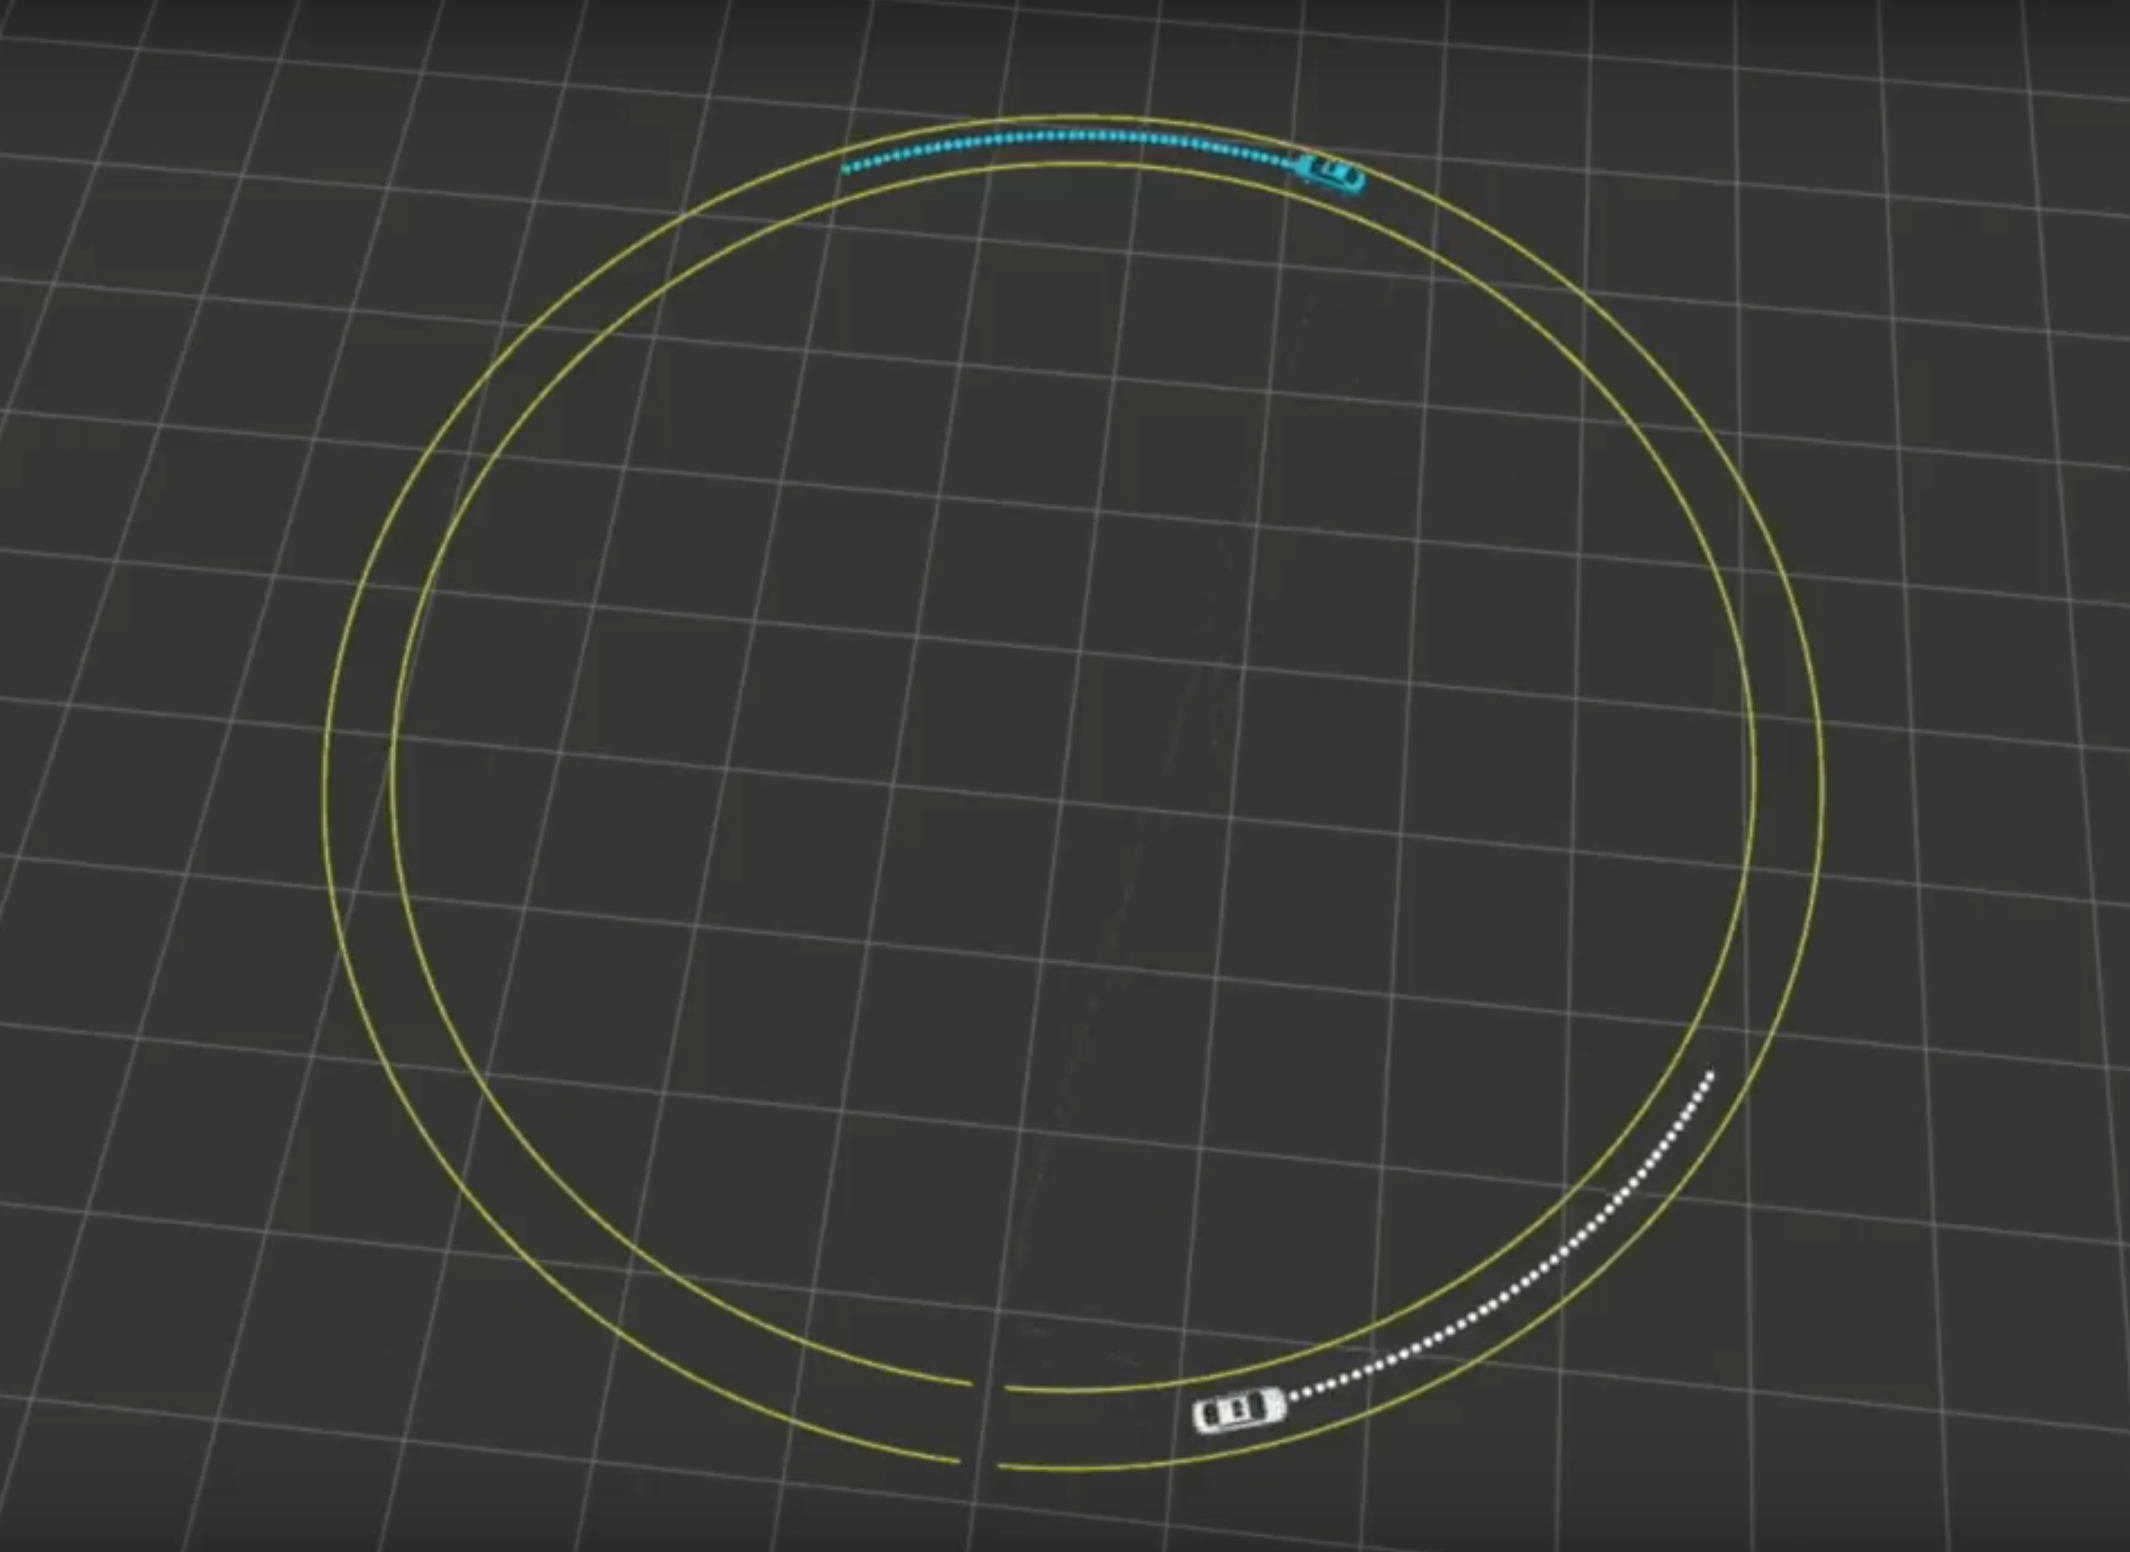
\includegraphics[width=1.0\textwidth]{figs/ch5/acc-env}
\caption{Training environment for Adaptive Cruise Control.}
\label{fig:acc-env}
\end{figure}

The neural network used for the DQN consists of the fully-connected layers with five hidden layers. RMSProp algorithm is used to minimize the loss with learning rate $\epsilon = 0.0005$. We set the size of the replay memory to 10,000. We set the replay batch size to 32. The summary of the DQN configurations used for our experiments is provided below:

\begin{itemize}
\item State buffer size: n = 3
\item Network architecture: fully-connected feed-forward network
\item Nonlinear function: leaky ReLU
\item Number of nodes for each layers : [3 (Input layer), 100, 70, 50, 70, 100, 5 (Output layer)]
\item RMSProp optimizer with learning rate 0.0005
\item Replay memory size: 10,000
\item Replay batch size: 32
\end{itemize}

The parameters are set as below,

\begin{itemize}
\item Cruise speed of the preceding vehicle is $v_{pre} = 10 m/s$ .
\item Safety distance is $dist_{safety} = 10 m$
\item $accel_{high}, accel_{low}, keep_{zero}, decel_{low}, decel_{high} = {2, 1, 0, -1, -2} m/s^2$
\end{itemize}

The reward function is as in \ref{eq:reward-func1} and we set $\alpha = 1.0$ and $\beta = 2.0$. 

\begin{itemize}
 \item $r_s$ = incremental travel distance from the last time step (we can simply use euclidean distance between the current position and the previous one since the time is short and curve road can be ignored)
 \item $r_{action}$ = \{accelerate or decelerate with 2 m/s: -1.0, accelerate or decelerate with 1 m/s: -0.5, keep the speed: 0.0\}
 \item $r_{collision}$ = \{No collision: 0.0, Collision: -100\}
\end{itemize}


\begin{figure}[h]
\centering
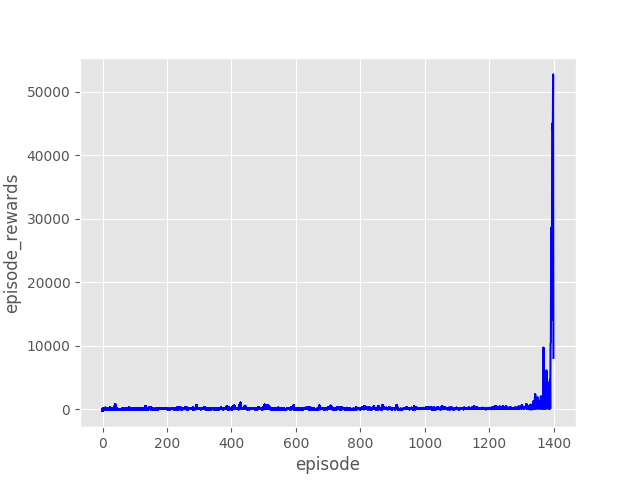
\includegraphics[width=1.0\textwidth]{figs/ch5/acc-reward}
\caption{The reward history of training for Adaptive Cruise Control.}
\label{fig:acc-reward}
\end{figure}

Fig. \ref{fig:acc-reward} provides the plot of the total accumulated rewards i.e., value function achieved for each episode. After 200 episodes, there shows a high jump of the reward which means ACC is working and it takes a long time to see a collision.

%%%%%%%%%%%%%%%%%%%%%%%%%%%%%%%%%%%%%%%%%%%%%%%%%%%%%%%%%%%%%%%%%
\section{Training for Combined Motion}

The ``combined motion" means that changing the speed and changing lanes are both available as driving behaviors. This environment with two lanes as shown in Fig. \ref{fig:auto-env} would focus on training an Adaptive Cruise Control and Lane Control agent for the ego vehicle. The ego vehicle and the other two vehicles would be initialized with defined the positions and headings and surely the relative position is enough safe. The dimension of the state space is set to $n = 5$ and the variables are the velocity of the ego vehicle $v_{ego}$, the longitudinal distance of the vehicles $s_{rel}$, the relative velocity $v_{rel} = v_{pre} - v_{ego}$, the flag showing if the left lane is available $flag_{left}$ and the flag showing if the left lane is available $flag_{right}$. To accelerate the training, they are normolized before feeding to the network.

\begin{figure}[h]
\centering
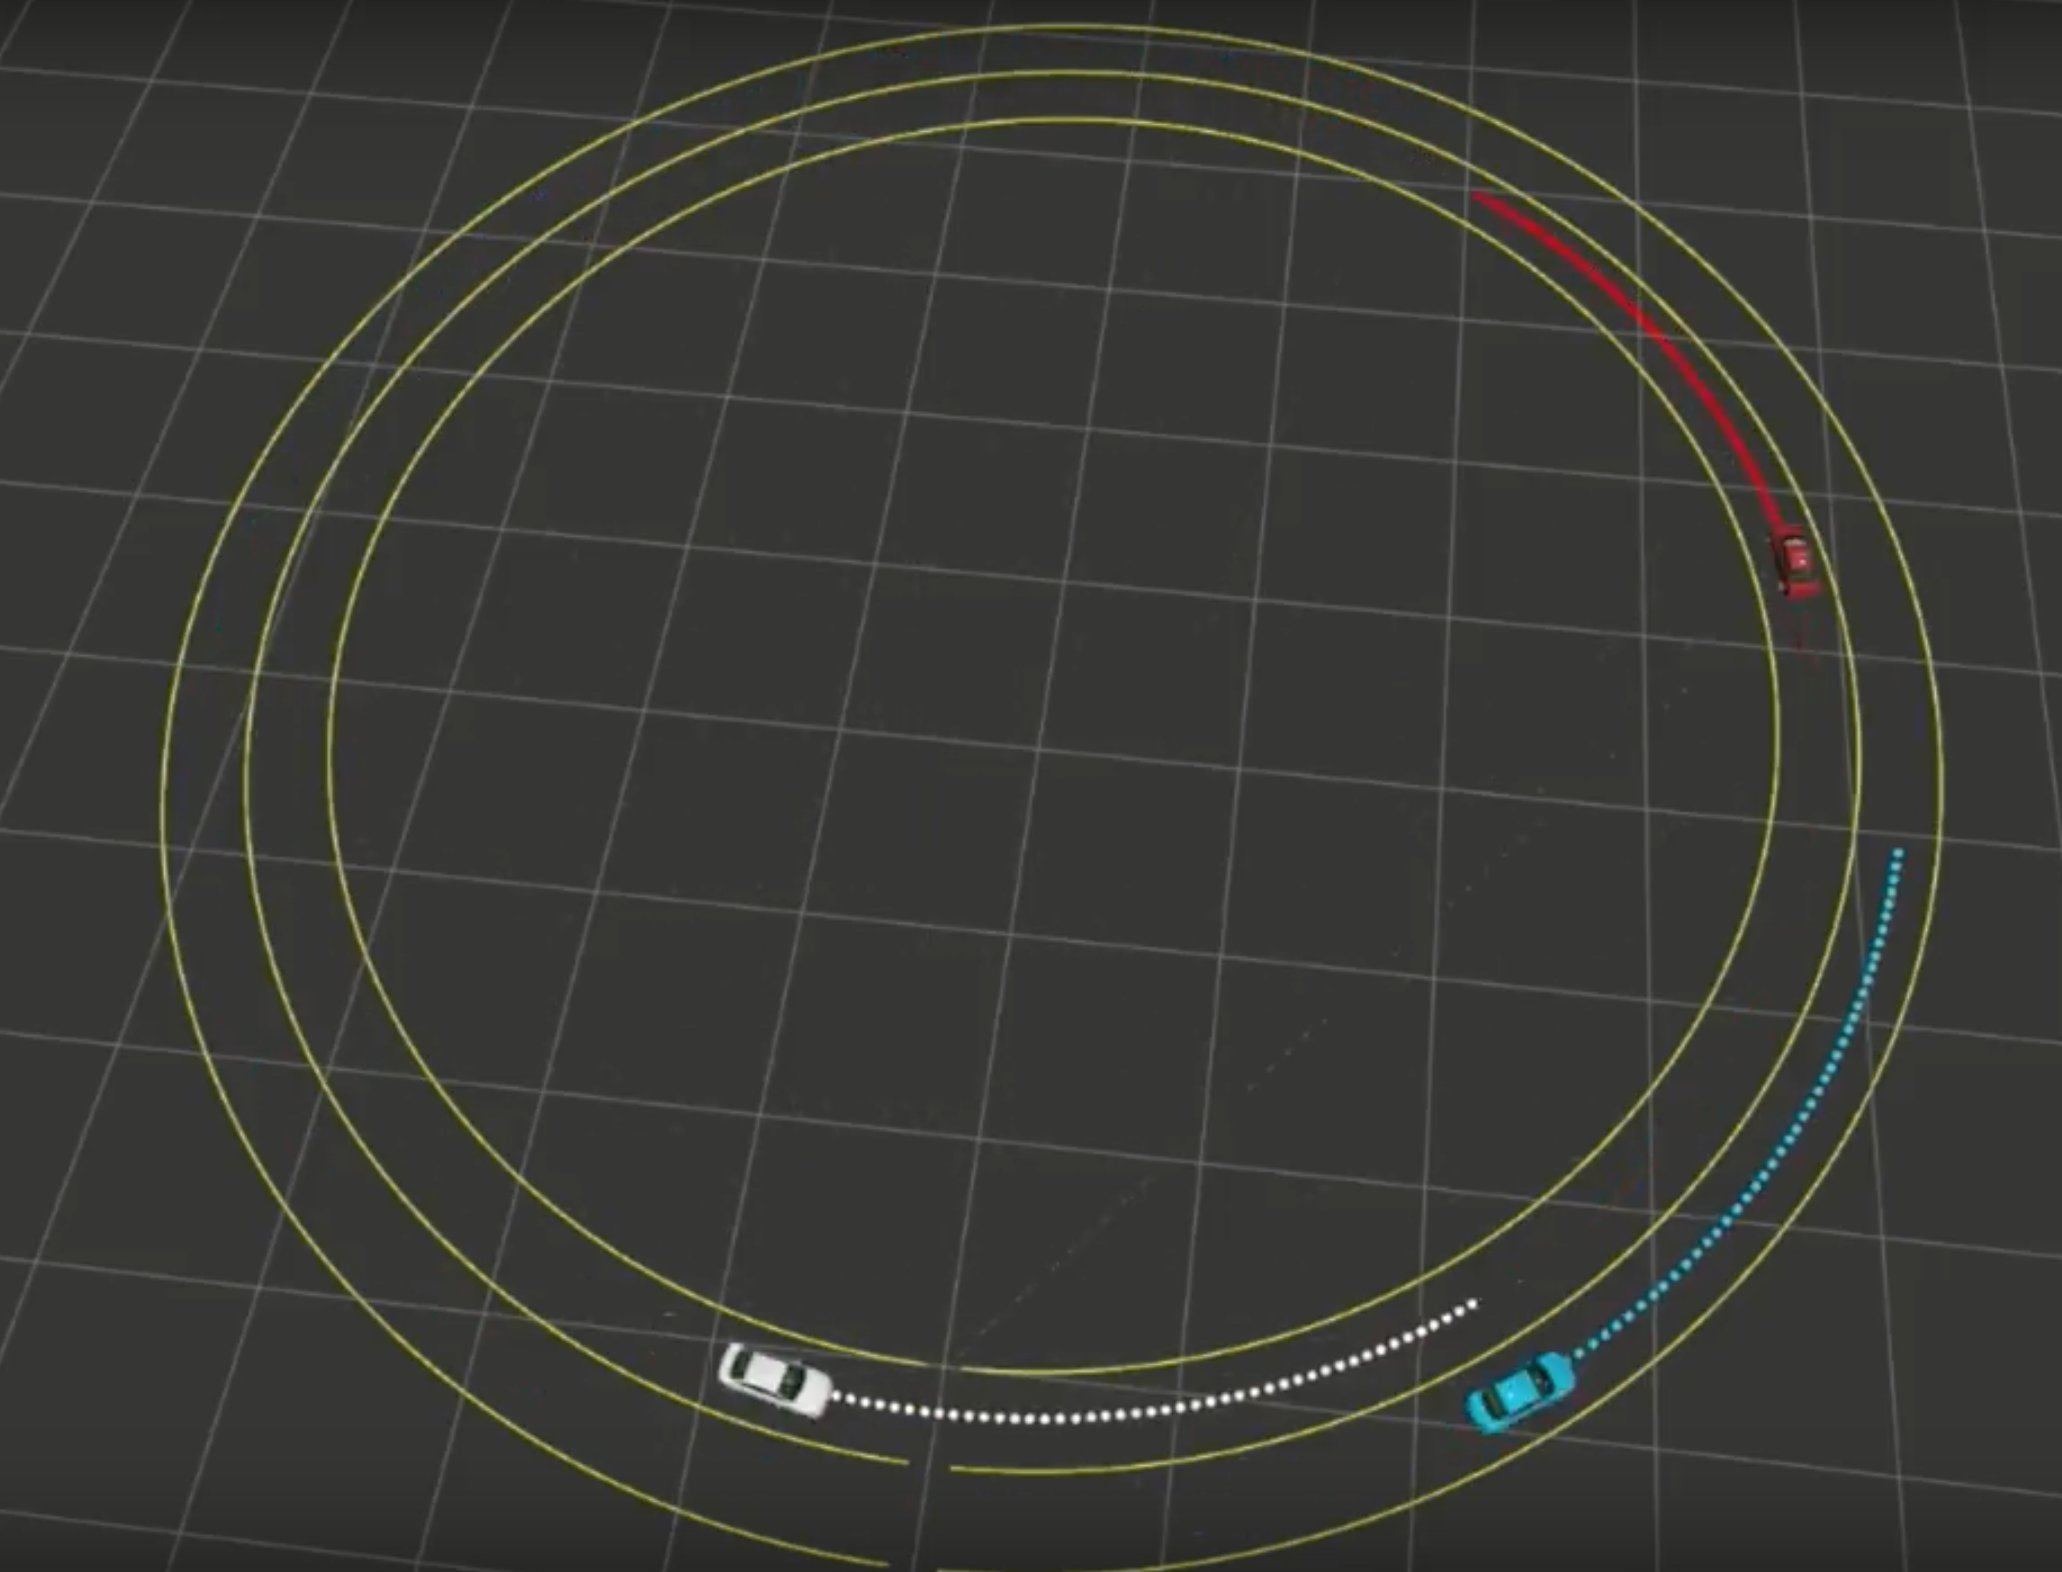
\includegraphics[width=1.0\textwidth]{figs/ch5/auto-env}
\caption{Training environment for Adaptive Cruise Control.}
\label{fig:auto-env}
\end{figure}

The summary of the DQN configurations used for our experiments is provided below:

\begin{itemize}
\item State buffer size: n = 5
\item Action Space size: $7 = 5 + 2$. (5 level of speed control and 2 modes of lane change)
\item Network architecture: fully-connected feed-forward network
\item Nonlinear function: leaky ReLU
\item Number of nodes for each layers : [5 (Input layer), 100, 70, 50, 70, 100, 7 (Output layer)]
\item RMSProp optimizer with learning rate 0.0005
\item Replay memory size: 10,000
\item Replay batch size: 32
\end{itemize}

The parameters are set as below,

\begin{itemize}
\item Cruise speeds in Lane 0 and 1 are $v_{lane0}, v_{lane1}$ = $6 m/s$, $5 m/s$, which means Lane 0 and 2 are Fast Lane and Slow Lane.
\item Safety distance is $dist_{safety} = 10 m$
\item $accel_{high}, accel_{low}, keep_{zero}, decel_{low}, decel_{high}$ = $2 m/s^2$, $1 m/s^2$, $0 m/s^2$, $-1 m/s^2$, $-2 m/s^2$.
\end{itemize}

The reward function is as in \ref{eq:reward-func2} and we set $\alpha = 1.0$, $\beta = 2.0$ and $\phi = 5.0$. 

\begin{itemize}
 \item $r_s$ = travel distance from the last time step (we can simply use euclidean distance between the current position and the previous one since the time is short and curve road can be ignored)
 \item $r_{action}$ = \{accelerate or decelerate with 2 m/s: -1.0, accelerate or decelerate with 1 m/s: -0.5, keep the speed: 0.0, change lane to left or right: -1.0\}
 \item $r_{lanechange}$ = \{Successful lane change: 0.0, Fail to change lane: -1.0\}
 \item $r_{collision}$ = \{No collision: 0.0, Collision: -100\}
\end{itemize}

\begin{figure}[h]
\centering
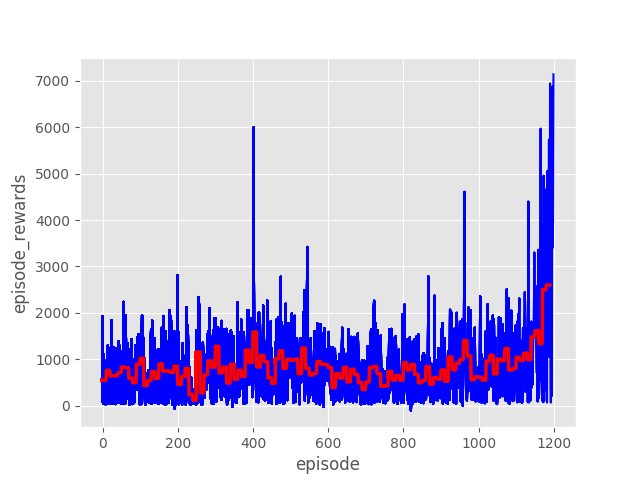
\includegraphics[width=1.0\textwidth]{figs/ch5/auto-reward}
\caption{The reward history of training for full autonomous highway driving.}
\label{fig:auto}
\end{figure}

Fig. \ref{fig:auto} provides the plot of the total accumulated rewards i.e., value function achieved for each episode. We observe that the value function converges after 2,000 episodes and high total reward is steadily attained after convergence.

\section{Main Evaluation}

Both $Agent1_{FCNN}$ and $Agent2_{FCNN}$ successfully drove the ego vehicle safely without collisions for a very long time and distance after enough training. Naturally, $Agent1_{FCNN}$ solved a significantly higher fraction of the episodes and performed better than $Agent2_{FCNN}$, since it only needed to control the speed, and not decide when to change lanes. In the beginning, it learned to always stay in its position to avoid an immediate collision, but quickly met a limit in receiving higher reward. With more training, it started to maintain a relatively high speed and keep stable if there is a preceding vehicle detected, but sometimes caused collisions. $Agent2_{FCNN}$ needs much more training to stay safe. A longer training run could be carried out for better performance.
